\documentclass[ALICE,manyauthors]{ALICE_internal_notes}
%\documentclass[ALICE,manyauthors]{ALICE_scientific_notes}

\usepackage {amsmath}
\usepackage {amssymb}
\usepackage {graphicx}
\usepackage {subfigure}
\usepackage {bm}
\usepackage {indentfirst} %indent the first par after section
\usepackage{setspace} 
\usepackage{color}

\RequirePackage{lineno}
\setlength{\linenumbersep}{6pt}
%\linenumbers

\newcommand{\slfrac}[2]{\left.#1\right/#2}
\usepackage{rotating}

\include{defs}

%------------------------------------------------------------------------------------
\begin{document} 
%------------------------------------------------------------------------------------

\begin{titlepage}
%
%\EXPnumber{ALICE-INT-2012-xxx} %\EXPdate{31 October 2011}
%\PHdate{\today}


\title{Run, track selection, efficiency correction for jet transverse momentum spectra analysis in \pp \s=2.76 , 7\tev\ and \ppb\ \s=5.02\tev\ collisions}
\ShortTitle{}   

\author{D.J.~Kim}%$^{1}$
\author{
%1. 
Jyv\"askyl\"a University and Helsinki Physics Institute, Finland\\
}
\author{Email: djkim@jyu.fi}
%
\ShortAuthor{ALICE Internal Note 2012}      % appears on left page headers, do not change
%
\begin{abstract}

\end{abstract}

\end{titlepage}
%%%%%%%%%%%%%%%%%%%%%%%%%%%%%%%%%%%%%%%%%%%%%%%%%

\tableofcontents

\clearpage


%%%%%%%%%%%%%%%%%%%%%%%%%%%%
\section{Introduction}
\label{sec:intro}
%%%%%%%%%%%%%%%%%%%%%%%%%%%%
All the analysis presented here are analyzed via the ALICE legotrain framework, where the location of the code is PWGCF/Correlation/JCORRAN in Aliroot  and the details of the real data and MC data sets
can be found the legotrain system. 
%%%%%%%%%%%%%%%%%%%%%%%%%%%%
\section{List of Data sets}
\label{sec:runlist}
Here I list  all the data sets and the corresponding legotrain ID for each analysis.
\begin{table}[ht]
\caption{List of Data sets used in the analysis.} 
\begin{center}
\begin{tabular}{| l | p{7cm}|| l  p{4cm}| |}
\hline
legotrain &   Data set  &  legotrain ID \\
\hline
CF\_pp    &      2760GeV\_LHC11a\_p4\_AOD113\_noSDD     & 511\_20141031\-1000 \\
CF\_pp    &      2760GeV\_LHC11a\_p4\_AOD113\_withSDD   & 521\_20141031\-1051 \\
CF\_pp    &      Full\_pp\_data\_set\_7TeV\_pass3\_LHC10b      & 519\_20141031\-1008 \\
CF\_pp    &      Full\_pp\_data\_set\_7TeV\_pass3\_LHC10c      & 520\_20141031\-1009 \\
CF\_pp    &      Full\_pp\_data\_set\_7TeV\_pass2\_LHC10d      & 517\_20141031\-1006 \\
CF\_pp    &     7TeV\_LHC10c\_p2\_AOD147                           & 514\_20141031\-1003 \\
CF\_pp    &     7TeV\_LHC10e\_p2\_AOD147                           &516\_20141031\-1005  \\
CF\_pPb  &     LHC13b\_pass3  & 573\_20141024\-1505 \\
CF\_pPb  &     LHC13c\_pass2  & 574\_20141024\-1505 \\
CF\_pPb  &     LHC13d\_pass2  & 575\_20141024\-1505 \\
CF\_pPb  &     LHC13e\_pass2  & 576\_20141024\-1505 \\

\hline
\end{tabular}
\end{center}
\label{tab:tunes}
\end{table}    

%%%%%%%%%%%%%%%%%%%%%%%%%%%%


%%%%%%%%%%%%%%%%%%%%%%%%%%%%
\section{Track selection cuts}

We have used the following charged particle track selection cuts based on the ALICE AOD track filter bit selection.
The naming and fiter bit for each track selection are shown in table~\ref{tab:treackfilterbit}.
The details on AOD track filter bit can be found at the twiki page\footnote{https://twiki.cern.ch/twiki/bin/viewauth/ALICE/PWGPPAODTrackCuts}.
\label{sec:tracks}
%%%%%%%%%%%%%%%%%%%%%%%%%%%%
\begin{table}[ht]
\caption{Track selections} 
\begin{center}
%enum { kJTPCOnly, kJRaa, kJGlobalTightDCA, kJGlobalDCA, kJGlobalSDD , kJHybrid, kJNTrackCuts };
\begin{tabular}{c|l}
\hline
cut name    &   AOD filter bit \\
\hline
TPCOnly    & 7 \\
Raa		  & 10 \\
Hybrid        & 8 or 9 \\
GlobalTightDCA & 5 \\
GlobalDCA         & 4 \\
GlobalSDD         & 5 or 6 \\
\hline
\end{tabular}
\end{center}
\label{tab:treackfilterbit}
\end{table}    


\newpage


%%%%%%%%%%%%%%%%%%%%%%%%%%%%
\section{Efficiency corrections}
\label{sec:eff}
%%%%%%%%%%%%%%%%%%%%%%%%%%%%
\label{sec:efficiency}
 Monte Carlo production cycles which were analyzed in order to study reconstruction efficiency
are listed in \tab{tab:tunes}. Estimate of track reconstruction efficiency and event selection efficiency 
follows the approach discussed in Section 6.2 of \cite{JFthesis}.

\begin{table}[ht]
\caption{Monte Carlo simulations} 
\begin{center}
\begin{tabular}{| l | p{7cm}|| l  p{4cm}| |}
\hline
Period   &   Tune  & lego train \\
\hline 
\pp\ 2.76\tev  & \small{LHC12f1a\_Pythia\_2760GeV}    & \small{CF\_pp\_MC212\_20141015} \\
		     & \small{LHC12f1b\_Phojet\_2760GeV}    & \small{CF\_pp\_MC213\_20141015} \\
\hline
\pp\ 7\tev  & \small{Pythia\_Full\_pp\_data\_set\_7\_TeV\_LHC10d1}    & \small{CF\_pp\_MC229\_20141024} \\
		& \small{Pythia:\_Full\_pp\_data\_set\_7.0\_TeV\_LHC10d4}    & \small{CF\_pp\_MC227\_20141024} \\
		& \small{Pythia6:\_Full\_pp\_data\_set\_7.0\_TeV\_LHC10f6a} & \small{CF\_pp\_MC226\_20141024} \\
		& \small{Pythia:\_Full\_pp\_data\_set\_7.0\_TeV\_LHC10e20} & \small{CF\_pp\_MC228\_20141024} \\
		     
\hline
\ppb 5.02\tev & \small{LHC13b2\_efix\_p1,2,3,4}  &  \small{CF\_pPb\_MC\-193(5,6,7)\_20141010} \\
\hline
\end{tabular}
\end{center}
\label{tab:tunes}
\end{table}    


Based on simulated inelastic events
we studied reconstruction efficiency of charged physical primaries selected with cuts
listed in \tab{tab:treackfilterbit}.
Charged physical primaries are  particles produced in a collision including the products of strong 
and  electromagnetic decay and excluding the feed-down from weak decays of strange particles.
The simulation tunes listed in \tab{tab:tunes} were used to get the relation between the number of charged
 physical primaries and the number of charged reconstructed tracks.
Charged physical primaries were identified using the AliRoot function IsPhysicalPrimary. 
Only those charged particles that were emitted to the range $|\eta| < 0.8$ were considered.
 In case of \pp{} and  \ppb{}  collisions event vertex $z$ coordinate was constrained to $\left|z_{vertex}\right|<10$~cm.  

Single track \emph{overall reconstruction correction} takes into account
\begin{itemize}  
\item contamination of the reconstructed track sample with fake primary tracks,
\item track reconstruction efficiency,
\end{itemize}
In following equations $G_{\rm trigvtx}$ stands for the number of true charged physical primaries emitted to  $|\eta|<0.8$
in triggered events where an event vertex was reconstructed. 
Similarly to \cite{JFthesis}, we define the track-to-particle \emph{overall reconstruction correction} 
 $C\left(\pt{}\right)$, 
\begin{eqnarray}
  C^{-1}\left( \pt{} \right)&=& { M_{\rm trigvtx}\left(\pt{}\right)+ B\left(\pt{}\right) \over   G_{\rm trigvtx} \left(\pt{}\right)},
 \label{eq:overallC}
\end{eqnarray}

Here $M_{\rm trigvtx}$ denotes the number of properly reconstructed primary tracks\footnote{ 
Reconstructed track that  passed the selection cut  had to have
 an absolute value of assigned label  equal to a label of some MC particle from the input
 MC sample of physical primaries, i.e., charged primary particles emitted to $|\eta|<0.8$.}
and $B$ gives the number of fake and secondary tracks. Let us point out that $G_{\rm trigvtx}$ and $M_{\rm trigvtx}$ are  functions 
of the original MC generator \pt{} while $B$ is a function of the reconstructed \pt{}.
We assume that reconstruction correction of the trigger and associated particle are independent.
Furthermore, we plot also the true track reconstruction efficiency and contamination which are defined as 
\begin{eqnarray}
  \mathrm{ true\,\, efficiency\,} &=&   M_{\rm trigvtx}\left(\pt{}\right)/G_{\rm trigvtx} \left(\pt{}\right), \\
  \mathrm{contamination} &=&  B\left(\pt{}\right)/ \left[  M_{\rm trigvtx}\left(\pt{}\right)+ B\left(\pt{}\right) \right] .
  \label{eq:Cont}
\end{eqnarray}
These ratios tell us what is the probability that an input MC charged primary track is reconstructed  and passes the selection  cuts   and
  what is the fraction of fake  primary tracks among all reconstructed tracks, respectively. 
  Overall reconstruction corrections, the true track reconstruction efficiency and contamination are shown in \fig{fig:eff_LHC13} for \ppb, \fig{fig:eff_LHC11a} for \pp \s=2.76\tev\ and \fig{fig:eff_7tev} for \pp \s=7\tev, respectively.
 
 \subsection{Trigger Efficiency}
In order to cross-check the efficiency correction we will compare charged track \pt{} spectra obtained
from this analysis with the results of the GSI group. For this purpose we have to normalize the \pt{}
spectrum per one inelastic event.

The total number of inelastic events equals
\begin{equation}
  N_{\rm inel} = \sum_{n=0}^{\infty} \int dz  I\left(z,\, n\right)
\end{equation}
where $I\left(z,\, n\right)$ gives the number of inelastic events having the number of contributors to a reconstructed
vertex equal to $n$ and the true MC vertex position in some range $(z,z+dz)$. The events where an interaction vertex was not reconstructed
have $n=0$ by definition.

The number of inelastic events with a reconstructed vertex ($n>0$) can be estimated as
\begin{equation}
I\left(z,\, n\right) = E^{*}_{\rm trigvtx}\left(z,\, n\right)\tilde{C}_{\rm vtx}\left(z,\,n\right)\,\tilde{C}_{\rm trig}\left(z,\,n\right)
\end{equation}
where $E^{*}_{\rm trigvtx}\left(z,\, n\right)$ stands for the measured number of triggered events with a reconstructed vertex
and $\tilde{C}_{\rm vtx}\left(z,\,n\right)$ and $\tilde{C}_{\rm trig}\left(z,\,n\right)$ denote corrections on
vertex reconstruction efficiency and trigger efficiency, respectively. Both correction factors are assessed
based on simulation
\begin{eqnarray}
 \tilde{C}_{\rm vtx} \left(z,\, n\right)&=& { E_{\rm trig} \left(z,\, n\right) \over  E_{\rm trigvtx} \left(z,\, n\right)},\\
 \tilde{C}_{\rm trig} \left(z,\, n\right)&=& { E_{\rm all} \left(z,\, n\right) \over  E_{\rm trig} \left(z,\, n\right)}
\end{eqnarray}
where  $E_{\rm class} \left(z,\, n\right)$ represents the number of inelastic events obtained from MC generator corresponding
to one of the event classes quoted in \tab{tab:class}.

In case that vertex was not reconstructed ($n=0$), we have
\begin{equation}
  I\left(z,\, 0\right) = E^{*}_{\rm trig}\left(0\right)  \alpha^{*} \left(z\right) F\left(z\right)\,\tilde{C}_{\rm trig} \left(z,\,0\right)\,.
\end{equation}
Here $E^{*}_{\rm trig}\left(0\right)$ gives the measured number of events which triggered but where an
interaction vertex was not reconstructed. These events are then distributed in the vertex diamond according to
the measured distribution of vertex positions
\begin{equation}
\alpha^{*} \left(z\right)={ \sum_{n=1}^{\infty} E^{*}_{\rm trigvtx}\left(z,\, n\right)   \over
                            \sum_{n=1}^{\infty}\int dz E^{*}_{\rm trigvtx}\left(z,\, n\right)}\,.
\end{equation}
The function $F(z)$ is a MC based correction which relates the shape of vertex distribution in events where a vertex
was not reconstructed and  the vertex distribution from reconstructed vertices
\begin{equation}
F\left(z\right) = { E_{\rm trig}(z,\,0)/\int dz  E_{\rm trig}(z,\,0)   \over
\sum_{n=1}^{\infty} E_{\rm trigvtx}(z,\,n)/\sum_{n=1}^{\infty}\int dz  E_{\rm trigvtx}(z,\,n)
}\,.
\end{equation}

Simulated and real events were divided into
6 multiplicity bins ( $n=0$, 1, 2, 3, 4, 5 to $\infty$) and
8 bins in $z$ vertex position (bin borders -10, -6, -3, -1.5, 0, 1.5, 3, 6, 10~cm).
  
  % P+PB  5.02 TeV 
\begin{figure}[p]
  \centering
  \resizebox{0.42\columnwidth}{!}{\includegraphics{./figs/CorrectionFactor_pPb.pdf}}
  \resizebox{0.42\columnwidth}{!}{\includegraphics{./figs/PureEfficiency_pPb.pdf}}
  \resizebox{0.42\columnwidth}{!}{\includegraphics{./figs/Contamination_pPb.pdf}}
  \caption{Top: Inverse of the overall reconstruction correction of reconstructed charged tracks  selected with various cuts.
   Middle: Corresponding true efficiency. Bottom: Corresponding contamination. 
    Data are from the MC tune.
 }
  \label{fig:eff_LHC13}
\end{figure}

  % P+ P  2.76 TeV 
\begin{figure}[p]
  \centering
  \resizebox{0.42\columnwidth}{!}{\includegraphics{./figs/CorrectionFactor_pp276.pdf}}
  \resizebox{0.42\columnwidth}{!}{\includegraphics{./figs/PureEfficiency_pp276.pdf}}
  \resizebox{0.42\columnwidth}{!}{\includegraphics{./figs/Contamination_pp276.pdf}}
  \caption{Top: Inverse of the overall reconstruction correction of reconstructed charged tracks  selected with various cuts.
   Middle: Corresponding true efficiency. Bottom: Corresponding contamination. 
    Data are from the MC tune.
 }
  \label{fig:eff_LHC11a}
\end{figure}

% P+ P  7 TeV 
\begin{figure}[p]
  \centering
  \resizebox{0.42\columnwidth}{!}{\includegraphics{./figs/CorrectionFactor_7TeV_GlobalDCA.pdf}}
  \resizebox{0.42\columnwidth}{!}{\includegraphics{./figs/CorrectionFactor_7TeV_GlobalTightDCA.pdf}}
  \resizebox{0.42\columnwidth}{!}{\includegraphics{./figs/CorrectionFactor_7TeV_GlobalSDD.pdf}}
  \caption{Top: Inverse of the overall reconstruction correction of reconstructed charged tracks  selected with various cuts.
   Middle: Corresponding true efficiency. Bottom: Corresponding contamination. 
    Data are from the MC tune.
 }
  \label{fig:eff_7tev}
\end{figure}


\newpage

%%%%%%%%%%%%%%%%%%%%%%%%%%%%
\subsection{Comparison of charged track \pt{} spectra with the published result}
\label{sec:spectracomparison}

We compare our inclusive spectra to the published ALICE results for each data sets.
\ppb\ charged particle spectra from our analysis is compared with the published data~\cite{Abelev:2014dsa} in different bins of $\eta$ windows and good agreement is shown in Fig~\ref{fig:spectra_LHC13}.
\pp \s=2.76 and 7\tev spectra from our analysis is compared with the published data~\cite{Abelev:2013ala} and good agreement for 7 \tev\ and ~5\% difference in 2.76\tev\ is observed and shown
in Fig~\ref{fig:spectra_LHC11a} and \ref{fig:spectra_7tev}. Since there is no Raa or Hybrid cut for MC tuned AOD for 7\tev, we have used 3 different sets of cuts available and difference among the cut variations
are below few \% level.

  % P+PB  5.02 TeV 
\begin{figure}[p]
  \centering
  \resizebox{0.45\columnwidth}{!}{\includegraphics{./figs/pPb_ALICEpT_eta_0.pdf}}
  \resizebox{0.45\columnwidth}{!}{\includegraphics{./figs/pPb_ALICEpT_eta_1.pdf}}
  \resizebox{0.45\columnwidth}{!}{\includegraphics{./figs/pPb_ALICEpT_eta_2.pdf}}
  \caption{The spectra from this analysis in \ppb \s = 5.02\tev\  is compared with the published ALICE data~\cite{Abelev:2014dsa}.}
  \label{fig:spectra_LHC13}
\end{figure}

  % P+P  2.76 TeV 
\begin{figure}[p]
  \centering
  \resizebox{0.52\columnwidth}{!}{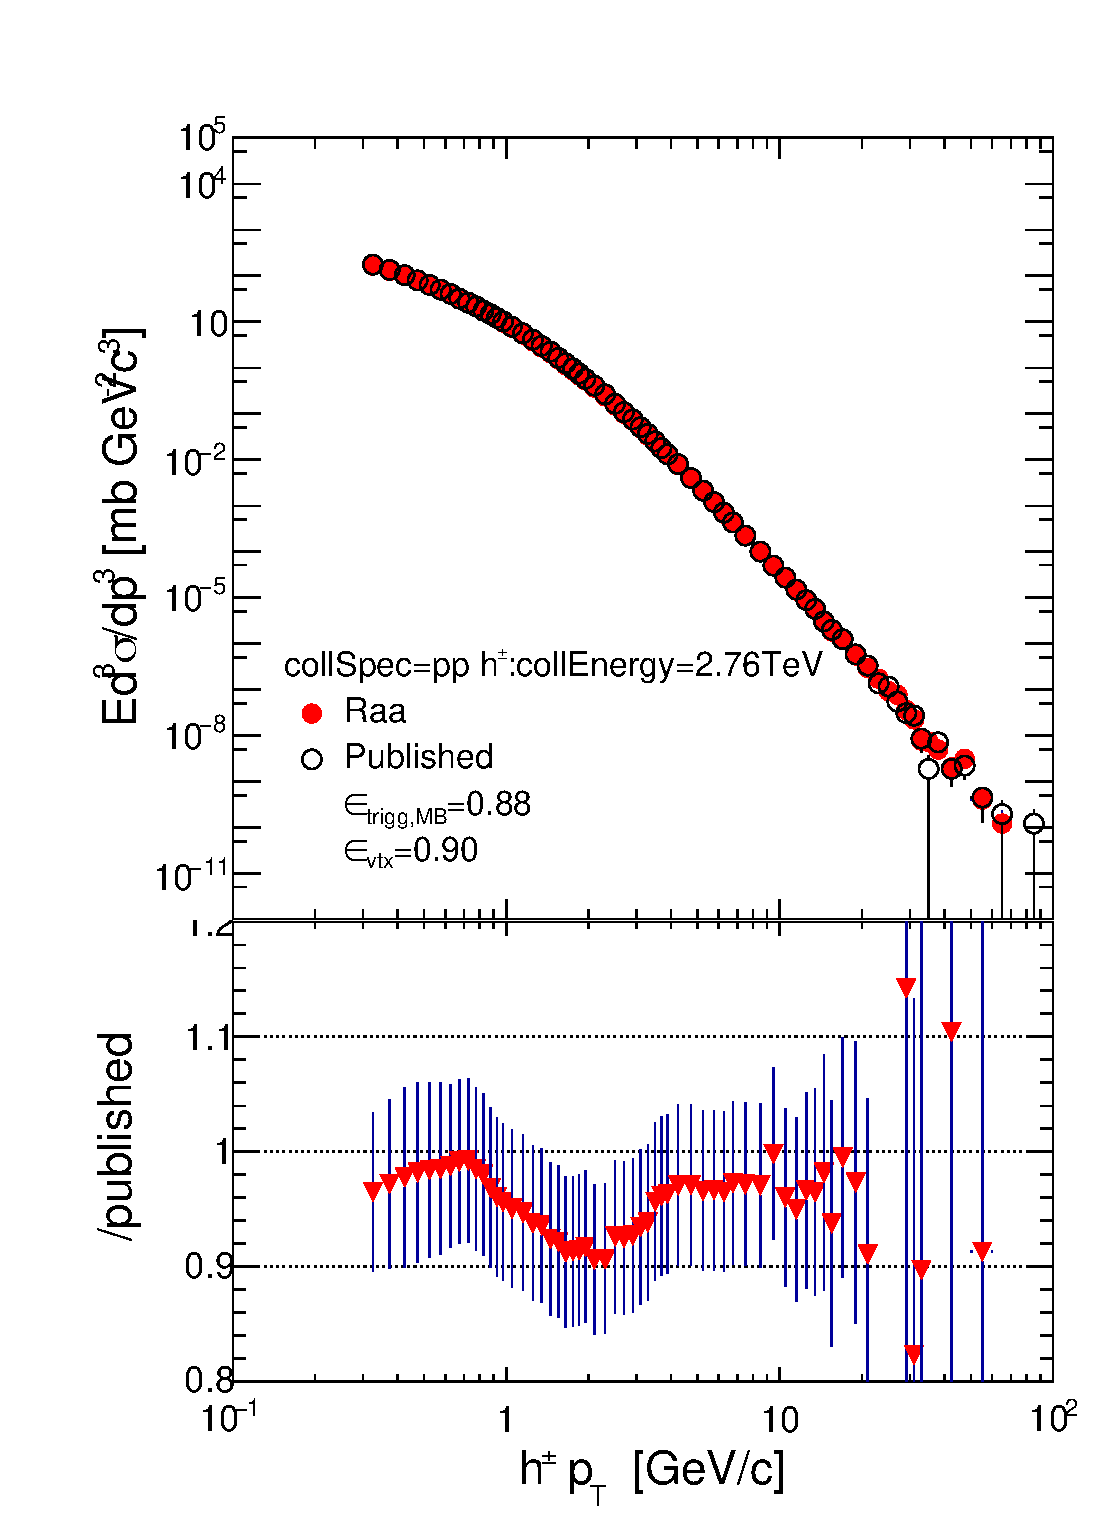
\includegraphics{./figs/invarJacek_pp276_withSDD.pdf}}
  \caption{The spectra from this analysis in \pp{} \s = 2.76\tev  is compared with the published ALICE data~\cite{Abelev:2013ala}.
 }
  \label{fig:spectra_LHC11a}
\end{figure}


  % P+P 7 TeV 
\begin{figure}[p]
  \centering
  \resizebox{0.32\columnwidth}{!}{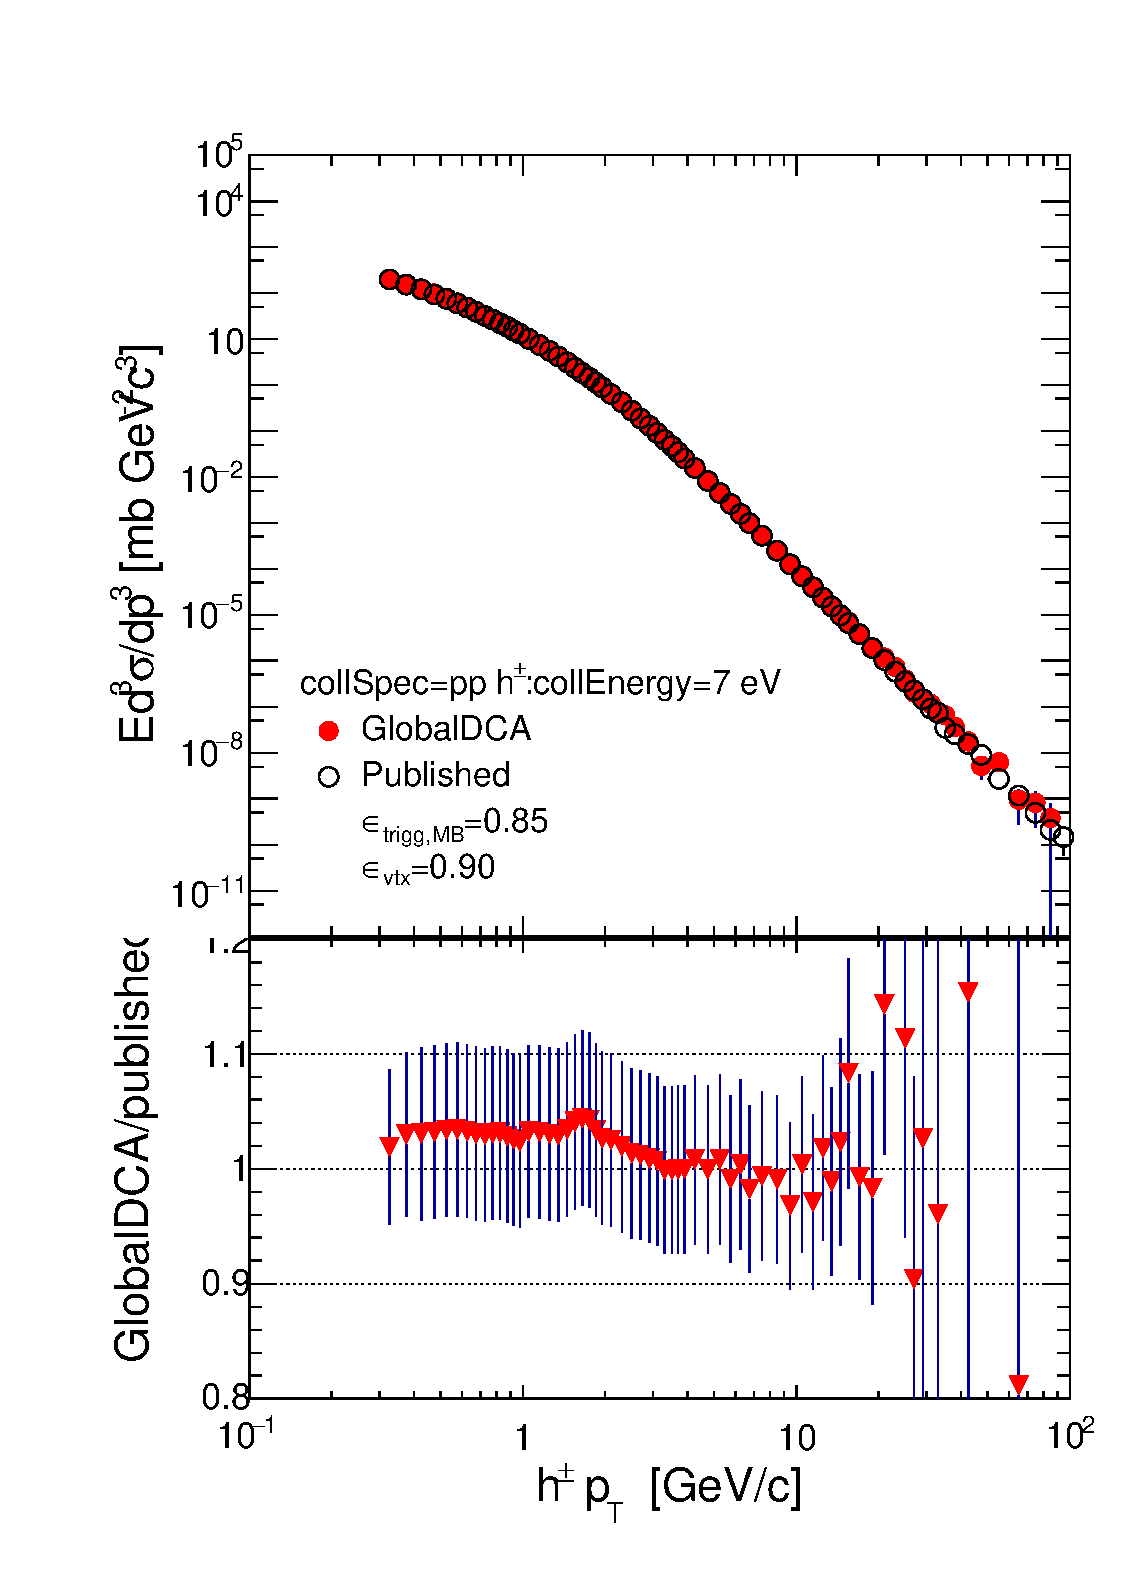
\includegraphics{./figs/invarJacek_pp_7TeV_C0_GlobalDCA.eps}}
  \resizebox{0.32\columnwidth}{!}{\includegraphics{./figs/invarJacek_pp_7TeV_C0_GlobalTightDCA.eps}}
  \resizebox{0.32\columnwidth}{!}{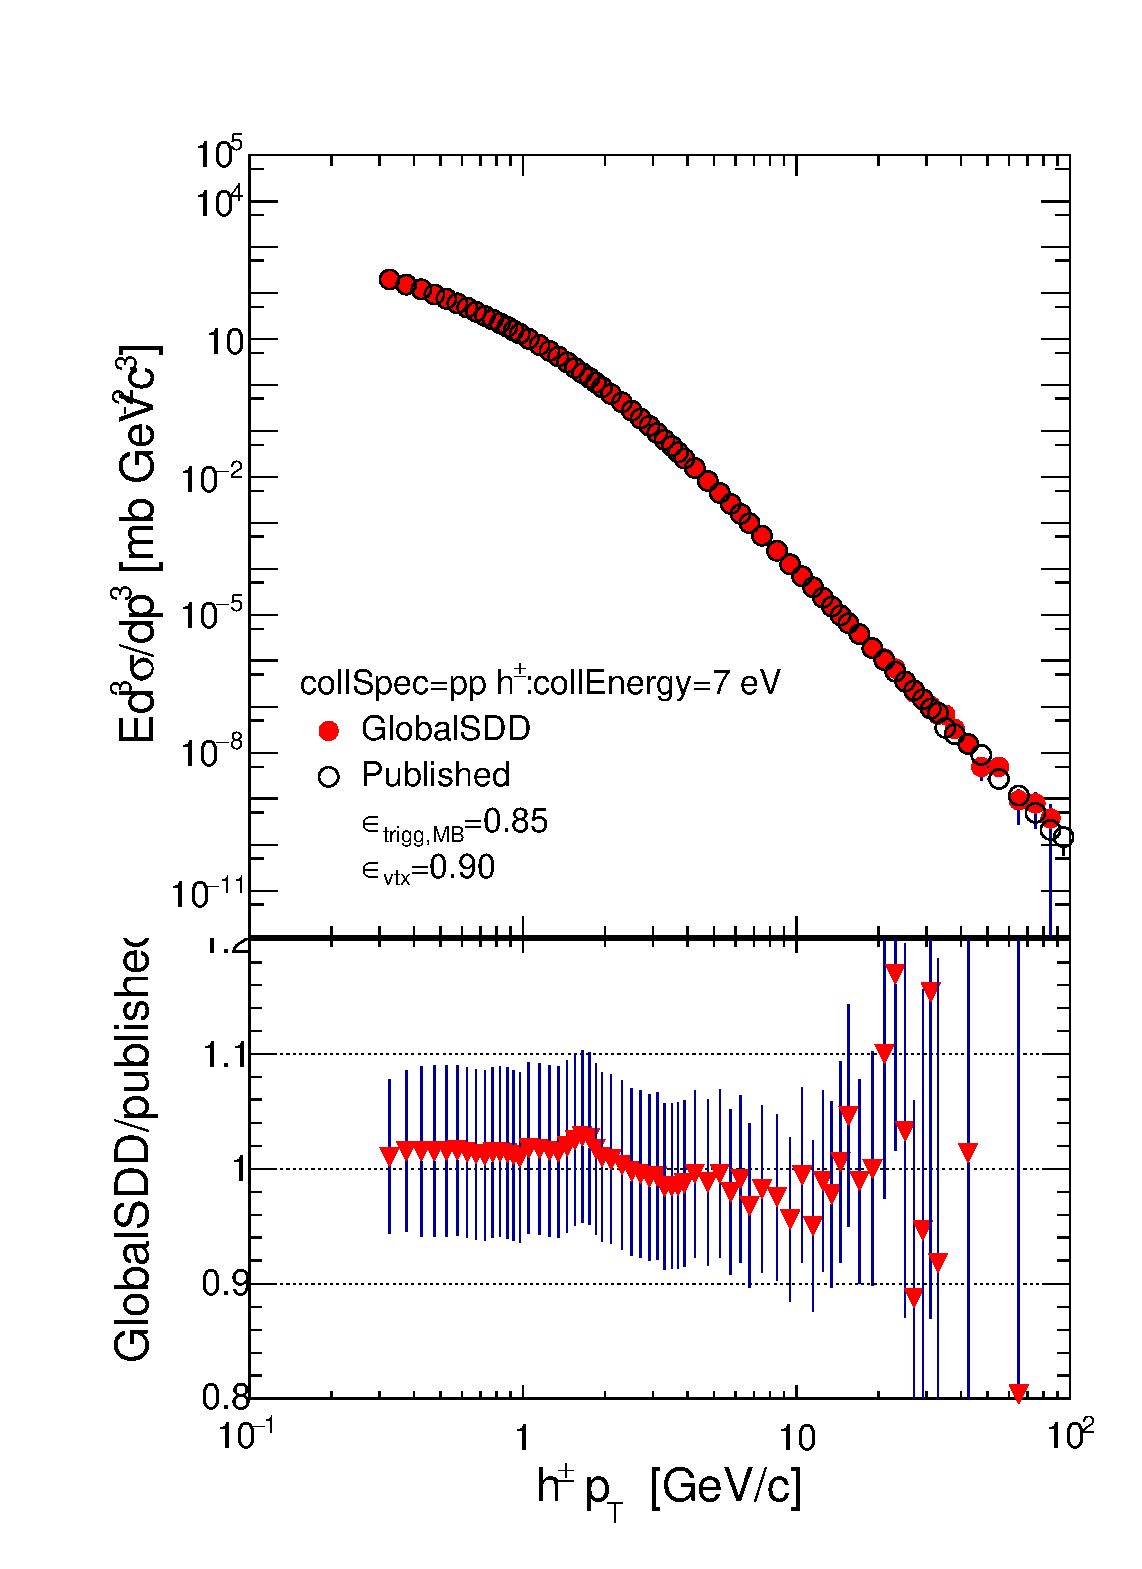
\includegraphics{./figs/invarJacek_pp_7TeV_C0_GlobalSDD.eps}}
  \caption{The spectra from this analysis in \pp{} \s = 7\tev\  is compared with the published ALICE data~\cite{Abelev:2013ala}.
 }
  \label{fig:spectra_7tev}
\end{figure}

%%%%%%%%%%%%%%%%%%%%%%%%%%%%
\label{sec:spectra}


\clearpage
\newpage

\bibliographystyle{prsty}
\begin{thebibliography}{9}
%\bibliographystyle{h-physrev3}
%\bibliography{/Users/janrak/papers/bib-mypapers,/Users/janrak/papers/bib-ALICE,/Users/janrak/papers/bib-ATLAS,/Users/janrak/papers/bib-CMS}
\bibitem{JFthesis}  J.F. Grosse-Oetringhaus,  \emph{Measurement of the Charged-Particle Multiplicity in Proton+Proton Collisions with the ALICE Detector},  CERN-THESIS-2009-033.
\bibitem{IaaAN}  A.Adare. ,  J.F. Grosse-Oetringhaus, A. Morsch,  \emph{ Azimuthal Correlations  in Pb+Pb Collisions}, AN version 5, 5 Sep. 2011. 
\bibitem{PRLiaa} Phys. Rev. Lett. 108, 092301 (2012).
\bibitem{Abelev:2014dsa} Eur. Phys. J. C 74 (2014) 3054, \emph{Transverse momentum dependence of inclusive primary charged-particle production in p-Pb collisions at $\sqrt{s_\mathrm{{NN}}}=5.02~\text {TeV}$}
\bibitem{Abelev:2013ala} 
  B.~B.~Abelev {\it et al.}  [ALICE Collaboration],
  %``Energy Dependence of the Transverse Momentum Distributions of Charged Particles in pp Collisions Measured by ALICE,''
  Eur.\ Phys.\ J.\ C {\bf 73}, 2662 (2013)
  [arXiv:1307.1093 [nucl-ex]].
  %%CITATION = ARXIV:1307.1093;%%
  %20 citations counted in INSPIRE as of 06 Nov 2014
\end{thebibliography}

\end{document}

